\chapter{Preface}\label{chap:preface}

A copy of this document and of all of its source code can be found at
\url{https://github.com/redpanda1234/thesis-public}.

Given the scope of this project, despite our best efforts, there are
probably a few typos. If any are spotted, we highly encourage the
reader to
\href{https://github.com/redpanda1234/thesis-public/issues}{submit an
  issue report}\footnote{URL:
  \url{https://github.com/redpanda1234/thesis-public/issues}} or
contact the author directly at
\href{mailto:fkobayashi@g.hmc.edu}{fkobayashi@g.hmc.edu}. Similarly if
one discovers any factual inaccuracies.



\section*{Notation}
% I just defined these commands because it wasn't worth the time to
% figure out why the kana were messing up line breaking in emacs
\newcommand{\hiragana}{ひらがな}
\newcommand{\katakana}{カタカナ}
We record some notational conventions used throughout this document.
First, a note on some non-standard glyphs:
\begin{leftbar}
  \textbf{Note:} we will sometimes make use of glyphs from the two
  Japanese phonetic alphabet systems, \hiragana\ (IPA:\footnote{See
    \href{https://en.wikipedia.org/wiki/International\_Phonetic\_Alphabet}{https://en.wikipedia.org/wiki/International\_Phonetic\_Alphabet}
    and
    \href{https://en.wikipedia.org/wiki/Help:IPA/Japanese}{https://en.wikipedia.org/wiki/Help:IPA/Japanese}}
  \ipa{\c{c}iRaga\textdownstep na}) and \katakana\ (IPA:
  \ipa{kataka\textdownstep na}). The motivation is that (a) more
  commonly-employed glyph systems (e.g., Greek / Roman) are heavily
  overloaded in mathematics, and (b) the \hiragana\ characters $つ$,
  $の$, $ゆ$, and $め$ look qualitatively similar to
  \begin{itemize}
    \item Planar isotopy (つ),
    \item Reidemeister I (の),
    \item Reidemeister II (ゆ), and
    \item Reidemeister III (め)
  \end{itemize}
  respectively, so they seemed a convenient alternative in the
  context of knot theory.

  It's worth mentioning that it's possible to typeset these symbols
  without having to use \XeLaTeX\ or \LuaLaTeX\ by using the
  \texttt{newunicodechar} package and manually specifying the code
  point in \texttt{udmj30}.\footnote{See
    \href{https://tex.stackexchange.com/a/171614}{https://tex.stackexchange.com/a/171614}}
  The author has made a small package for \LaTeX\ that does this; it
  can be found on
  \href{https://github.com/redpanda1234/kana.sty}{Github}.\footnote{\url{https://github.com/redpanda1234/kana.sty}}
\end{leftbar}



\subsection*{Table of Symbols}
{\footnotesize
  \begin{longtable}{@{}llr@{}}
    \toprule Notation \hspace{2cm} & Meaning \hfill & Page (if applc.)
    \\ \midrule
    $つ$ & Reidemeister ``0'' move (planar isotopy) & \\
    $の$ & Reidemeister I move & \\
    $ゆ$ & Reidemeister II move & \\
    $め$ & Reidemeister III move & \\
    $ラ$ & Generic Reidemeister move \\
    $ら$ & Alt.\ to ラ & \\
    \midrule
    $K$ & Generally reserved for knots & \\
    $\msf K$ & Generally reserved for \emph{polygonal} knots & \\
    $S^n$ & The standard $n$-sphere & \\
    $\mbb{D}^n$ & The standard $n$-ball ($\partial \mbb{D}^n =
    S^{n-1}$) & \\
    $\triangle$ & Used for simplices & \\
    $\ip{A}$ & Sometimes used for $\text{convex hull}(A)$ & \\
    \midrule
    $\spn{a,b}$ & Open interval in $S^1$ & \pageref{sec:s1-notation} \\
    $\sbk{a,b}$ & Closed interval in $S^1$ & \pageref{sec:s1-notation}\\
    $a \sprec b \sprec c$ & $b \in \spn{a,c}$ & \pageref{sec:s1-notation} \\
    % $\sbk{a,b}$ & Closed interval in $S^1$ & \pageref{sec:s1-notation}\\
    \midrule
    $\ms T_{\rm std}$ & The standard topology on $\RR^n$ & \\
    $\bk{a,b}$ & $\set{x \in \RR \MID a \leq x \leq b}$ & \\
    $\pn{a,b}$ & $\set{x \in \RR \MID a < x < b}$ & \\
    $B_r(x)$ & Ball of radius $r$ centered at $x$ & \\
    $\pn{x_{\alpha}}_{\alpha \in \square}$ & Seq.\ of $x$ indexed by
    $\alpha \in \square$ & \\
    $\pn{x_{\alpha}}_{\alpha \in \square} \subseteq X$ & Shorthand for
    a seq.\ of points in
    $X$. & \\
    $x_\alpha \incto x$ & $x_\alpha$ increase to $x$ & \\
    $x_\alpha \to x$ & $x_\alpha$ converges to $x$ & \\
    $x_\alpha \xrightarrow{u} x$ & $x_\alpha$ converges to $x$
    uniformly & \\
    $x_\alpha \decto x$ & $x_\alpha$ decrease to $x$ & \\
    \midrule
    $\ol{A}$ & Closure of $A$ & \\
    $A^c$ & Set complement of $A$ & \\
    $X \setminus A$ & $\set{x \in X \MID x \not \in A}$ & \\
    $X - A$ & Alt.\ to $X \setminus A$ & \\
    $A \subseteq X$ & $A$ is a subset of $X$ & \\
    $A \subsetneq X$ & $A$ is a proper subset of $X$ & \\
    \midrule
    $f : A \into B$ & $f$ is injective from $A$ to $B$ & \\
    $f : A \onto B$ & $f$ is surjective from $A$ to $B$ & \\
    $f : A \bij B$ & $f$ is a bijection between $A$ and $B$ & \\
    $f|_S$ & $f$ restricted to $S$ & \\
    $\fpre{f}{A}$ & Inverse image of $A$ under $f$ & \\
    $\overrightarrow{f}(A)$ & Image of $A$ under $f$ & \\
    \midrule
    $\ZZ^{> 0}$ & Positive integers & \\
    $\ZZ^{\geq 0}$ & Non-negative integers & \\
    $\RR^{> 0}$ & Positive reals & \\
    $\RR^{\geq 0}$ & Non-negative reals & \\
    $\ZZ_+$ & Alt.\ for $\ZZ^{>0}$ & \\
    $\RR_+$ & Alt.\ for $\RR^{>0}$ & \\
    \midrule
    $\mspace{-6mu}\st$ & Such that & \\
    $\jiong$ &
    Contradiction\footnote{\url{https://en.wiktionary.org/wiki/\%E5\%9B\%A7\#Chinese}} & \\
    $\blacksquare$ & QED & \\
    $\square$ & QED for small proofs (e.g.\ claims, sketches) & \\
    $\lozenge$ & Used to denote the end of definitions, etc. & \\
    \midrule

    {[IPA]} & Occasionally used for IPA pronuncation & \\
    \np{words} & Used to help parse large noun phrases & \\
    \bottomrule
  \caption{Some notational conventions}
  \label{tab:notation}
\end{longtable}}

% \end{table}

\subsection*{Flipbook}
A flipbook showing the construction of a $(7,2)$ knot has been
provided in the right margin for the reader's entertainment.


\subsection*{Document Formatting}\label{pref:formatting}
Throughout this document we will occasionally use a \emph{leftbar}
environment to visually distinguish some parts of the document from
others. E.g., in providing a recap of a series of proofs, we might do
something like
\begin{leftbar}
  \textbf{Recap:} The above results are rather technical, but they are
  important because Lemma 1 gives [\ldots], which will allow us to
  show [\ldots] later.
\end{leftbar}
If pursuing an iff proof, it will likely be formatted as follows:
\begin{iffproof}
  \item We want to show $A \implies B$. [\ldots]
  \item We want to show $B \implies A$. [\ldots]
\end{iffproof}
We mentioned this in the notation table, but we'll do so here again.
Sometimes, if there is a particularly nasty-to-parse noun phrase,
we'll wrap it in \np{tortoise shell brackets}\footnote{きっこ
  う(\ipa{kik\textcorner k\|`o:}).} to make the sentence easier to
read (we hope).

Finally, wherever possible, we have sought to insert hyperlinks for
cross-referenced material (e.g., theorems, citations, equations, etc.)
so that readers using a PDF copy can navigate it more easily. The
coloring scheme is the default for the \texttt{hyperref} package,
which is as follows.
\begin{itemize}
  \item Red for {\color{red} linkcolor},
  \item Black for {\color{black} anchorcolor},
  \item Green for {\color{green} citecolor},
  \item Cyan for {\color{cyan} filecolor},
  \item Red again for {\color{red} menucolor},
  \item Cyan again for {\color{cyan} runcolor}, and
  \item Magenta for {\color{magenta} urlcolor}.
\end{itemize}




% \begin{figure}[H]
%   \centering
%   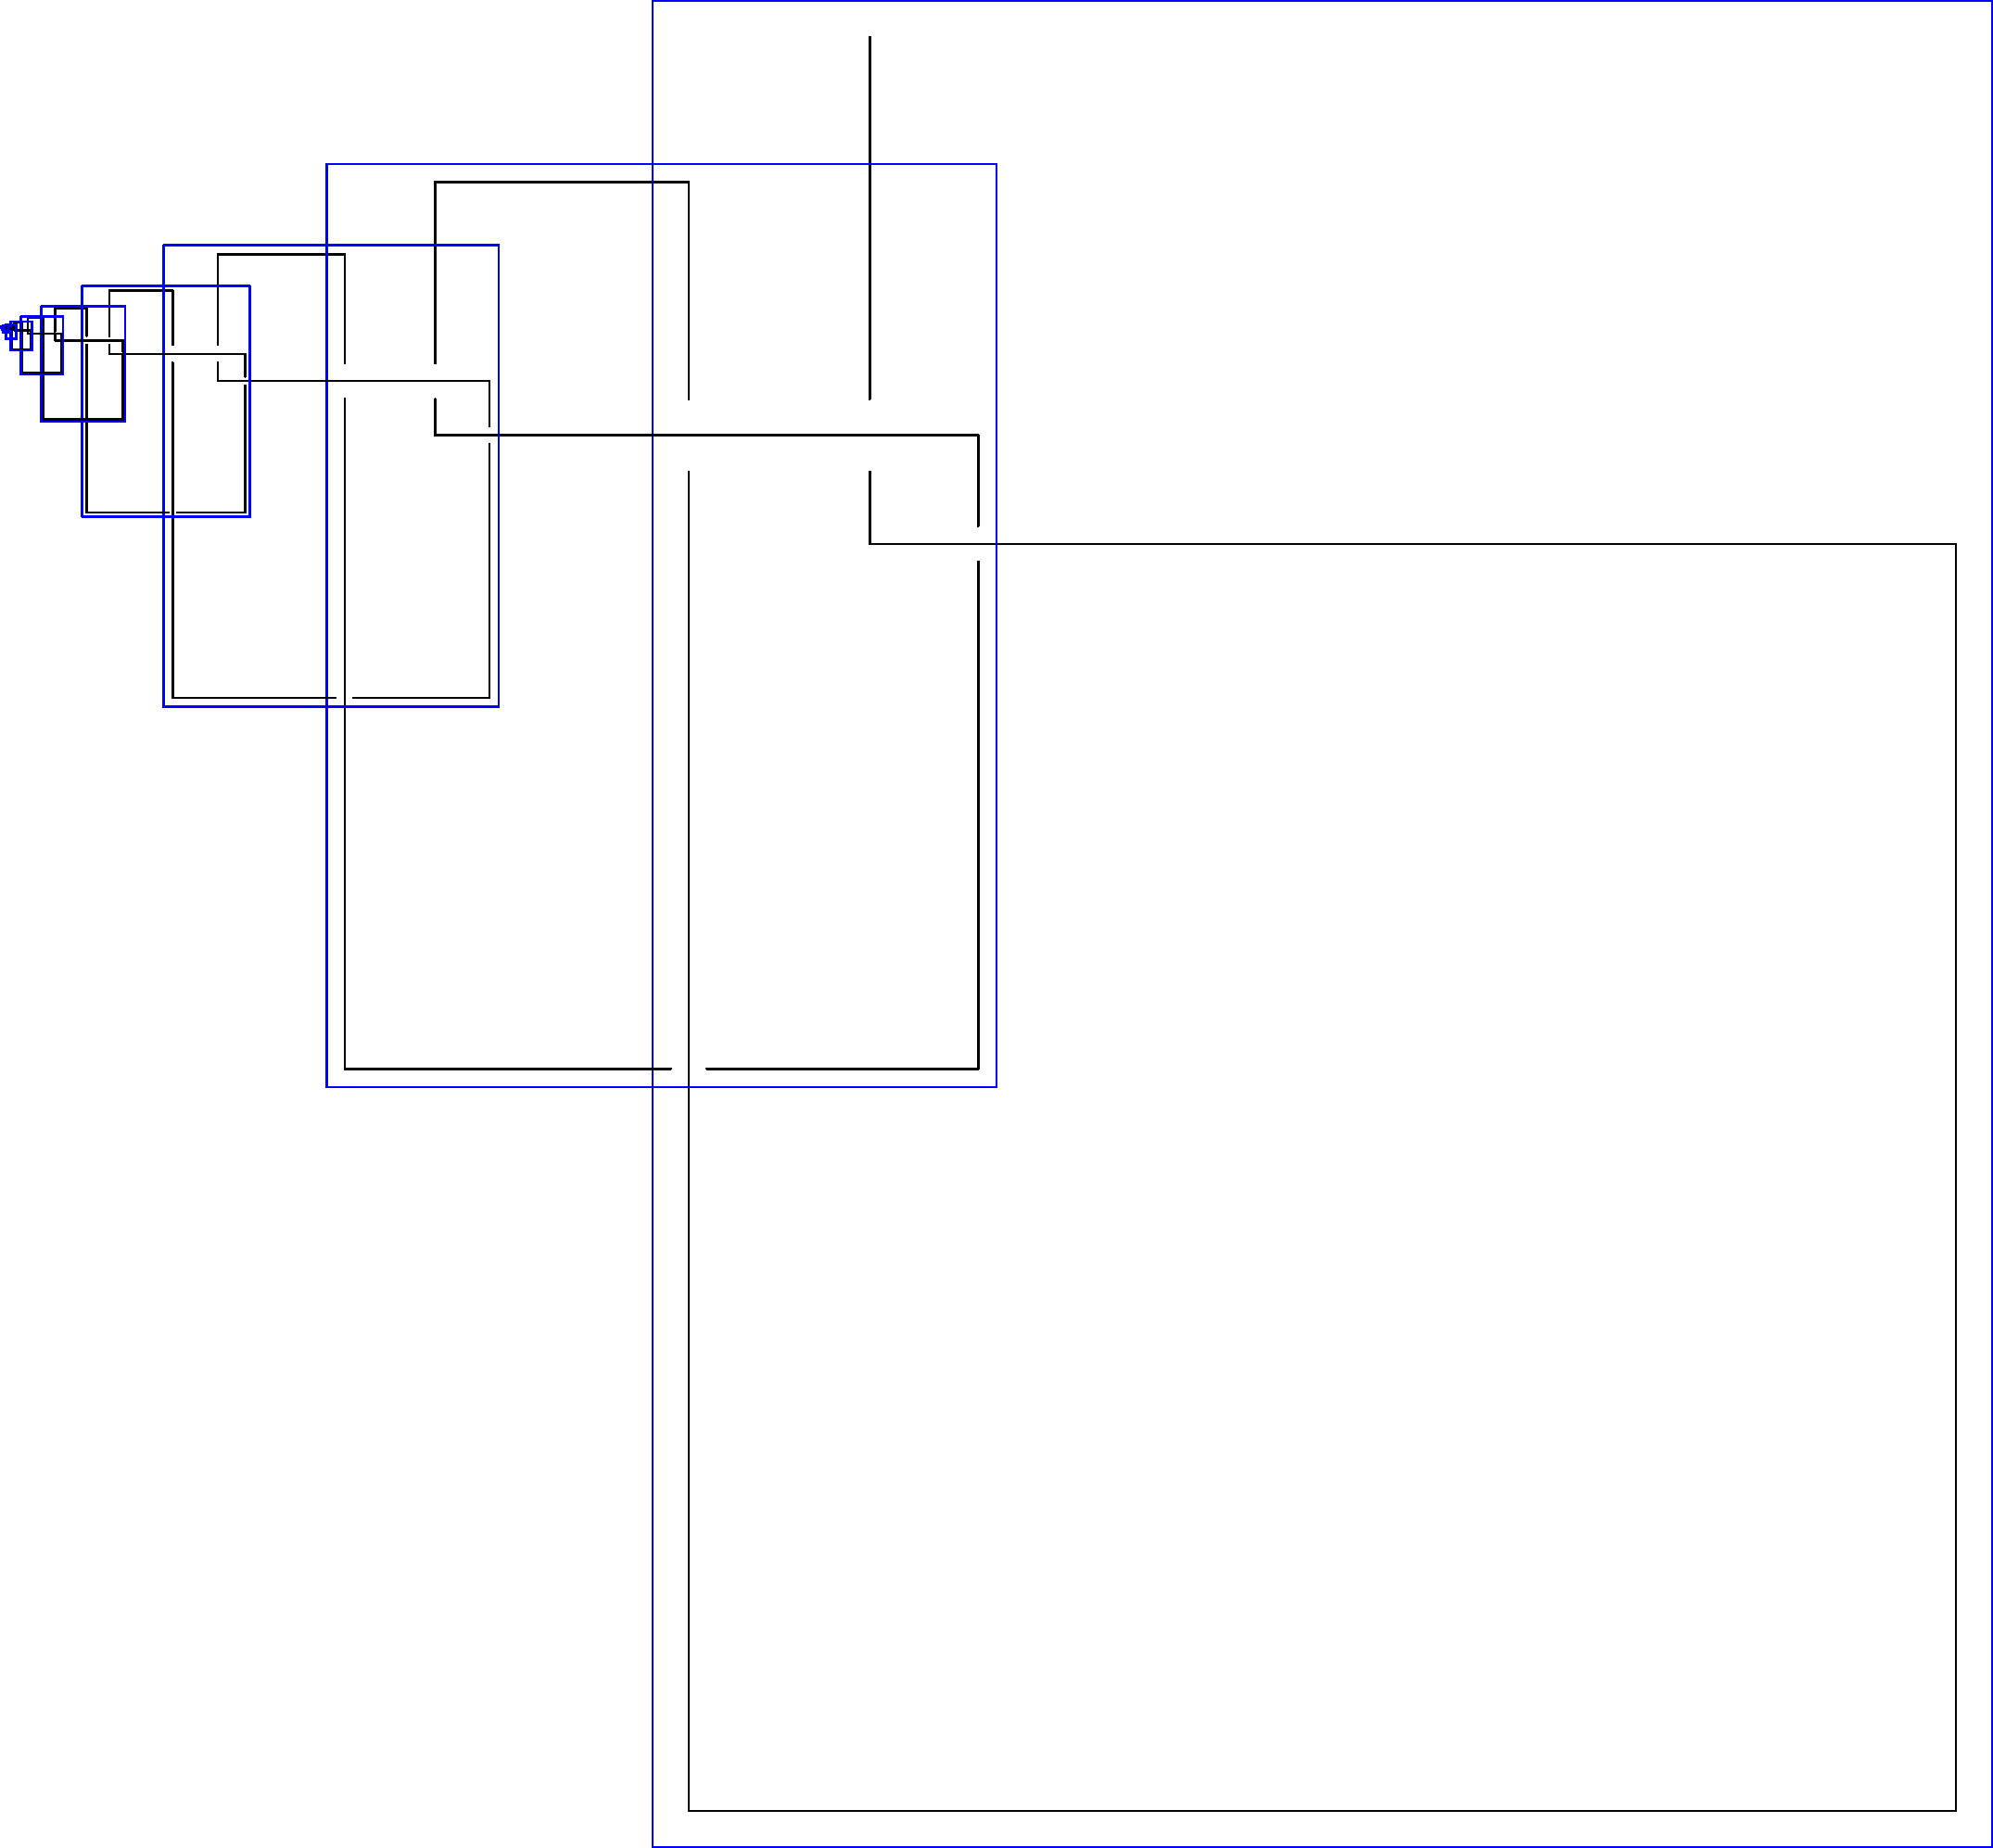
\includegraphics[scale=.2]{figures/preface/loops.pdf}
% \end{figure}


% The idea is to take a
% sequence of nested closed neighborhoods


%  set our attention on
% trying to understand existing literature on wild knots

% This led to a deep dive into the relationships between topological
% knots and their diagrams.

% Hence, phase II of the thesis could be best described as
% \begin{enumerate}[label=(\arabic*)]
%   \item
% \end{enumerate}

% The first plan of attack was to try and find a flaw in the uniform
% convergence argument. One was not immediately obvious to us, although
% this does not mean an error does not exist. Hence, we turned to


% As it turned out, this was also quite ambitious. In the past century
% almost all of the focus of the discipline of Knot Theory has been on
% tame knots. This presents a problem for our purposes,


% Of course, we claim that the example given above \emph{is
%   tame as well} --- the problem is that


% This led to a \emph{deep} foray into the foundations of knot theory,
% to find where the inconsistency lay.

% In particular, our example seemed to suggest an inconsistency between
% (\cref{def:cdef1}) and (\cref{def:cdef2} and \cref{def:cdef3}). To the
% best of our knowledge, this is not actually the case --- rather, the
% confusion seems to arise from hidden hypotheses and/or collisions in
% vocabulary. In \cref{def:cdef1}, we start with an arbitrary embedding
% $K : S^1 \into \RR^3$. In \cref{def:cdef2} and (with some further
% clarifying additions) \cref{def:cdef3}, we're implicitly working in
% the \emph{smooth} category --- meaning we require the knot $K$ to have
% a well-defined tangent vector at every point. This precludes
% embeddings like the one shown in \cref{fig:pref-strange-unknot}; it's
% unclear how to specify a well-defined tangent vector at the limit
% point of the loops.



% The loop nonsense above IS locally flat.

% For S^1 -> R^3, tame implies locally flat
% Hence, not locally flat -> not tame

% Part of the reason this took so long to discover was that as far as we
% can tell, the term \emph{piecewise linear} has been used
% inconsistently in the literature, {\color{green} and (worse still) on
%   StackOverflow!} In particular, sometimes the definition of
% \emph{piecewise-linear} is made in implicit reference to \emph{finite}
% simplicial complexes, and other times, it is made in reference to
% \emph{locally-finite} simplicial complexes.\footnote{If this is a
%   misunderstanding on the author's part, the reader is encouraged to
%   get in contact so that this characterization can be fixed!}


% But actually, the confusion doesn't stop there. As


% This
% led us to take an extended foray into the foundations of knot theory,
% ultimately shifting the focus of the project towards
% \begin{leftbar}
%   ``Seeking a better understanding of the relationships between knots
%   and knot diagrams, with a particular eye towards trying to find an
%   analog of Reidmeister's Theorem for wild knots.''
% \end{leftbar}

% \noindent \textbf{Common Definition 1} (Tame Knot):

% \noindent \textbf{Common Definition 2} (Tame Knot):

% \noindent \textbf{Common Definition 3} (Tame Knot):



%  to carefully examine the foundations of
% knot theory, and try and determine whether Reidemeister's theorem
% could be extended in way to knots with finitely-many wild points.

% \nomenclature{$c$}{Speed of light in a vacuum inertial frame}
% \nomenclature{$h$}{Planck constant}

% \printnomenclature

%%% Local Variables:
%%% TeX-master: "../../kobayashi-thesis"
%%% End:
